\documentclass[14pt]{extarticle}

\usepackage{geometry}
\geometry{a4paper,
          total={165mm,257mm},
          left=30mm,
          top=20mm,
         }

% \documentclass{article}

\usepackage[utf8]{inputenc}
\usepackage[T1, T2A]{fontenc}
\usepackage[english, russian]{babel}
\usepackage{csquotes}

\usepackage[
    backend = biber,
    style = numeric,
]{biblatex}

\addbibresource{Refs.bib}

\usepackage{graphicx}
\graphicspath{ {./images/} }

% \usepackage[table,xcdraw]{xcolor}

\usepackage{cmap}

\usepackage{hyperref}
\hypersetup{
    colorlinks=true,
    linkcolor=blue,
    filecolor=blue,
    urlcolor=blue,
    citecolor=blue,
    pdftitle={Отчёт о моделировании частотных сканов},
    pdfpagemode=UseOutlines,
    % pdfstartview={FitB}
}
\urlstyle{same}


\title{Моделирование частотных сканов}
\author{Богачёв А.М.}
\date{\today}


\begin{document}

    \maketitle

    \begin{abstract}
        В отчёте приведены результаты исследований...
    \end{abstract}

    \tableofcontents

    \section{Введение}
Релаксационная спектроскопия глубоких уровней (РСГУ) -- метод исследования 
электрически активных дефектов в полупроводниковых материалах. Данный метод 
обладает высокой чувствительностью к малым концентрациям ловушек носителей 
зарядов и является спектроскопическим. Существуют различные вариации РСГУ, 
например токовая и емкостная, так метод емкостной релаксационной спектроскопии 
глубоких уровней основан на исследовании процесса (сигнала) релаксации ёмкости 
барьерной структуры. Определив значения постоянной времени сигнала релаксации 
для разных температур образца, исследователь может определить энергию активации 
дефекта, вызывающего релаксацию. 

В идеальном случае релаксация ёмкости носит экспоненциальный характер, однако 
так бывает не всегда. Согласно обзору \cite{istratov_exp_analysis} 
сигналы релаксации ёмкости барьерных структур можно условно разделить на три 
группы:
    \begin{enumerate}
        \item Моноэкспоненциальный сигнал релаксации, обусловленный одним 
        единственным энергетическим уровнем в запрещённой зоне полупроводника.
        \item Сигнал релаксации, состоящий из суммы нескольких 
        моноэкспоненциальных сигналов релаксации.
        \item Сигнал релаксации, характеризуемый непрерывным распределением 
        скоростей эмиссии, представленным спектральной функцией $g(\lambda)$.
    \end{enumerate}
В последних двух случаях сигнал не является экспоненциальным. 

Задача определения постоянной времени одной или нескольких экспоненциальных 
составляющих процесса релаксации ёмкости или спектральной функции $g(\lambda)$ 
отностися к задачам экспоненциального анализа. Подходы к решению таких задач,
а также фундаментальные ограничения и особенности сбора и обработки 
экспериментальных данных рассмотрены в исчерпывающем обзоре 
\cite{istratov_exp_analysis}.

Во Владимирском Государственном университете создан измерительно-вычислительный
комплекс релаксационной спектроскопии глубоких уровней, основным измерительным
прибором которого служит спектрометр DLS"~82E фирмы Semilab. 
Измерительно-вычислительный комплекс реализует метод емкостной РСГУ с частотным
сканированием при постоянной температуре. В спектрометре аппаратно реализована
корреляционная обработка сигнала релаксации с опорной функцией lock-in. 

Технические решения, заложенные в названном измерительном оборудовании, требуют
особых методов анализа полученных экспериментальных данных, в частности,
разработки и идентификации моделей частотных сканов (экспериментальных данных, 
полученных на измерительно-вычислительном комплексе).

В следующих разделах отчёта будут рассмотрены модели частотных сканов, некоторые
технические и методические вопросы их реализации и идентификации, а также их
аппробация на экспериментальных данных.

% В современной учебной и технической литературе набирают популярность термины 
% <<машинное обучение>> и <<статистическое обучение>> (например в книгах 
% \cite{hands_on_ml}, \cite{nikolenko_deep_learning}, 
% \cite{elements_of_statistical_learning}). За ними, как правило, скрывается
% процесс создания моделей, которые после идентификации их параметров на некой
% тренировачной выборке (экспериментальных данных с известными целевыми 
% значениями), способны с некоторой точностью определять целевые значения для
% новых, ранее невстречавшихся данных. Таким образом, регрессия и классификация
% являются одними из самых частых задач машинного обучения \cite{hands_on_ml}.
% В данном отчёте термин <<машинное обучение>> будет использоваться именно для 
% обозначения процесса разработки и идентификации моделей, решения задачи 
% регрессии.

    \section{Математические модели частотных сканов}
    В данном разделе представленны описания математических моделей сигнала
    релаксации ёмкости и моделей частотного скана.


    \subsection{Модель сигнала релаксации ёмкости}
    Согласно обзору \cite{istratov_exp_analysis}, зависимость значения
    ёмкости от времени $f(t)$ для моноэкспоненциального сигнала релаксации
    имеет вид выражения \ref{eq:monoexp}.
    \begin{equation}
        \label{eq:monoexp}
        f(t) = A \exp \left(-\lambda t\right) ,
    \end{equation}
    где
    \begin{description}
        \item[\(A\)] -- амплитуда сигнала релаксации ёмкости;
        \item[\(\lambda\)] -- скорость экспоненциального спада,
        обратнопрпорциональная постоянной веремени сигнала релаксации
        $\tau$ (выражение \ref{eq:lambda}).
    \end{description}
    \begin{equation}
        \label{eq:lambda}
        \lambda = \tau ^ {-1}
    \end{equation}
    Спектр моноэкспоненциального сигнала релаксации имеет вид, 
    представленный на рисунке \ref{pic:monoexp_spect_example}.
    \begin{figure}[!ht]
        \centering
        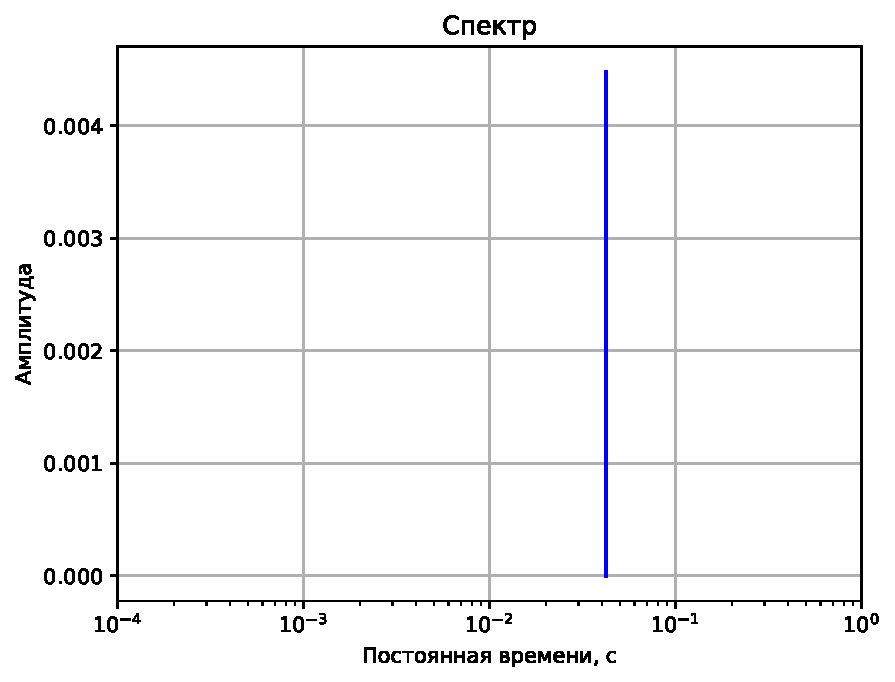
\includegraphics[width=0.5\textwidth]{monoexp_spect_expample}
        \caption{Пример спектра моноэкспоненциального сигнала релаксации
        ёмкости.}
        \label{pic:monoexp_spect_example}
    \end{figure}

    Согласно источнику \cite{istratov_exp_analysis}, зависимость сигнала 
    релаксации ёмкости от времени $f(t)$ для сгинала, образованного 
    несколькими дискретными экспоненциальными сигналами, определяется 
    выражением 
    \ref{eq:discr_multiexp}.
    \begin{equation}
        \label{eq:discr_multiexp}
        f(t) = \sum_{i=1}^{n}A_i\exp\left(-\lambda_i t\right) ,
    \end{equation}
    где $n$ -- количество экспоненциальных составляющих в спектре.
    Пример спектра такого сигнала показан на рисунке 
    \ref{pic:multiexp_spect_example}.
    \begin{figure}[!ht]
        \centering
        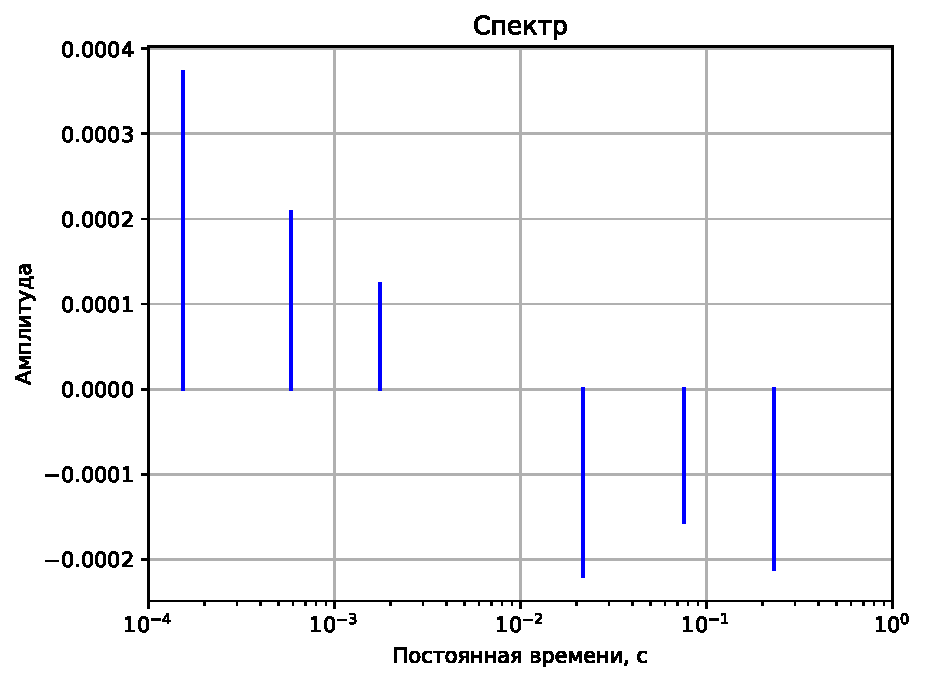
\includegraphics[width=0.5\textwidth]{multiexp_spect_example}
        \caption{Пример спектра сигнала релаксации ёмкости, содержащего
        несколько экспоненциальных составляющих.}
        \label{pic:multiexp_spect_example}
    \end{figure}


    \subsection{Модель идеального частотного скана}
    Предполагается, что в идеальном случае сигнал релаксации ёмкости содержит 
    одну экспоненциальную составляющую, а измерительный тракт спектрометка
    линеен. В таком случае модель частотного скана описывает аппаратные 
    преобразования спектрометра DLS"~82E учитывая только форму его опорной
    функции.

    В спектрометре DLS-82E реализована корреляционная обработка сигнала
    релаксации ёмкости, таким образом сигнал на выходе аналогового тракта
    спектрометра определяется выражением \ref{eq:dlts_correlation_tech},
    согласно публикации \cite{istratov_exp_analysis}.
    \begin{equation}
        \label{eq:dlts_correlation_tech}
        S\left[g(\lambda),t_c,t_d\right]=\frac{1}{t_c}\int_{t_d}^{t_d+t_c}
        f(t)W\left(t-t_d\right)dt ,
    \end{equation}
    где
    \begin{description}
        \item[$W(t)$] -- весовая функция, определённая на интервале 
        времени $\left[0,t_c\right]$,
        \item[$t_c$] -- период (длительность) весовой функции $W(t)$,
        \item[$t_d$] -- время задержки между началом сигнала релаксации
        и началом корреляционной обработки. Согласно обзору 
        \cite{istratov_exp_analysis}, время задержки $t_d$, обычно, 
        вводится для улучшения избирателности или для снижения искажения
        сигнала из-за перегрузки измерительной системы.
        \item[$g(\lambda)$] -- распределение скоростей экспоненциальных
        спадов, составляющих релаксационный сигнал.
    \end{description}

    Модель аппаратных преобразований (корреляционной обработки),
    учитывающая форму весовой функции, реализованной в спектрометре
    DLS"~82E, для моноэкспоненциального сигнала определяется выражением
    \ref{eq:dls82e_model_S} \cite{rp_vak}.
    \begin{equation}
        \label{eq:dls82e_model_S}
        S\left(\tau,C_A,F_0, t_1\right) = C_A K_{BS} K_{LS} 
        \phi\left(\tau,F_0,t_1\right),
    \end{equation}
    где
    \begin{description}
        \item[$C_A$] -- амплитуда емкостного релаксационного сигнала,
        \item[$K_{BS}$] -- масштабный коэффициент, зависящий от 
        чувствительности емкостного моста,
        \item[$K_{LS}$] -- масштабный коэффициент селектора,
        \item[$\tau$] -- постоянная времени релаксации глубокого уровня,
        \item[$F_0$] -- частота сканирования импульсов заполнения,
        \item[$t_1$] -- длительность импульса заполнения,
        \item[$\phi\left(\tau,F_0,t_1\right)$] -- функция определяемая
        выражением \ref{eq:dls82e_model_phi}.
    \end{description}
    \begin{equation}
        \label{eq:dls82e_model_phi}
        \phi\left(\tau,F_0,t_1\right) = 
        M \tau F_0 e^{-\frac{0.05}{\tau F_0}}
        \left(1-e^{\frac{t_1 F_0-0.45}{\tau F_0}}
        -e^{-\frac{0.5}{\tau F_0}}+
        e^{\frac{t_1 F_0-0.95}{\tau F_0}}\right),
    \end{equation}
    где $M$ -- масштабный множитель.

    Масштабный множитель $M$ определяется выражением
    \ref{eq:dls82e_model_M}.
    \begin{equation}
        \label{eq:dls82e_model_M}
        M(\tau, F_0, t_1) = \frac{1}{\max{\left[
        \tau F_0 e^{-\frac{0.05}{\tau F_0}}
        \left(1-e^{\frac{t_1 F_0-0.45}{\tau F_0}}
        -e^{-\frac{0.5}{\tau F_0}}+
        e^{\frac{t_1 F_0-0.95}{\tau F_0}}\right)
        \right]}}
    \end{equation}

    Введём коэффициент $A$ (выражение \ref{eq:dls82e_model_A}), 
    характеризующий амплитуду сигнала релаксации ёмкости и перепишем 
    выражение \ref{eq:dls82e_model_S} с учётом того, что длительность
    импульса заполнения $t_1$ является неизменной величиной, и получим
    выражение \ref{eq:dls82e_model_S_short}.
    \begin{equation}
        \label{eq:dls82e_model_A}
        A = C_A K_{BS} K_{LS}.
    \end{equation}
    \begin{equation}
        \label{eq:dls82e_model_S_short}
        S(\tau,A,F_0) = A\phi(\tau, F_0)
    \end{equation}


    \subsection{Модель, учитывающая нелинейность и неэкспоненциальность}

    Для одновременного учёта нелинейности аппаратного тракта и 
    неэкспоненциальности сигнала релаксации, связанной с присутствием 
    нескольких экспоненциальных составляющих в модель вводят коэффициент
    нелинейности"=неэкспоненциальности $p$ \cite{rp_vak}, после чего 
    выражение \ref{eq:dls82e_model_S_short} приобретает вид выражения 
    \ref{eq:dls82e_model_S_p}.
    \begin{equation}
        \label{eq:dls82e_model_S_p}
        S(\tau,A,F_0,p) = A\left[\phi(\tau, F_0)\right]^p.
    \end{equation}

    В случае моноэкспоненциального сигнала релаксации и линейного измерительного
    тракта коэффициент $p=1$, в остальных случаях он отклоняется от 1. Данный 
    коэффициент комплексно учитывает нелинейность и неэкспоненциальность, что
    позволяет повысить точность моделирования, но он не позволяет дать ответ 
    на вопрос какой именно из этих двух факторов имел место.


    \subsection{Модель многоэкспоненциального частотного скана}
    Если предположить, что сигнал релаксации ёмкости состоит из нескольких
    экспоненциальных составляющих и определяется выражением
    \ref{eq:discr_multiexp}, то опираясь на выражения
    \ref{eq:discr_multiexp}, \ref{eq:dlts_correlation_tech}, 
    \ref{eq:dls82e_model_S_short} и \ref{eq:dls82e_model_phi}, можно
    сделать выод, что частотный скан, созданный таким сигналом релаксации
    ёмкости определяется выражением~\ref{eq:multiexp_frequncy_scan}.
    \begin{equation}
        \label{eq:multiexp_frequncy_scan}
        Y = \sum_{i=1}^{n} A_i \phi(\tau_i, F_0) ,
    \end{equation}
    где $n$ -- количество экспоненциальных составляющих в сигнале 
    релаксации.
    Данная модель предполагает, что измерительный такт линеен.




    \printbibliography[heading=bibintoc, 
                       title={Список литературы}]

\end{document}